\subsection{Swath Processing}
\subsubsection{Raw Data and Waterfall Image Formation}
Side scan sonar data acquisition begins with the transmission of acoustic pulses and the recording of their backscattered echoes along each sonar beam. Each transmitted ping produces a 1D return signal that represents the intensity of acoustic reflections as a function of slant range. This signal corresponds to the strength of the backscattered energy received from the seafloor at varying distances from the transducer.  
\\ \\
As the vehicle moves forward, consecutive pings are recorded sequentially and combined to form a 2D intensity representation known as a \textit{``waterfall image''} or raw swath. In this format, the horizontal axis corresponds to the ping index or along track progression, while the vertical axis represents the across track slant range. The pixel intensity encodes the relative strength of the measured backscatter, providing an initial qualitative visualization of seafloor texture and reflectivity.  
\\ \\
This raw waterfall image forms the foundational representation of the side scan sonar data. However, it still remains in the sonars native measurement space, where each sample is indexed by slant range rather than by a geometrically corrected seabed location. As a result, the raw image is not yet directly suitable for consistent mapping or feature extraction, since vehicle attitude, transducer geometry, and acquisition conditions still affect the apparent structure of the swath.  
\\ \\
The subsequent stages of swath processing therefore aim to improve the physical consistency of each ping before later mapping stages. In this work, the swath processing stage focuses on geometric correction using the estimated vehicle pose and altitude, blind zone removal, and intensity normalization. Together, these steps produce a cleaner and more consistent swath representation that is suitable for later local map generation and feature extraction.
\begin{figure}[H]
    \centering
    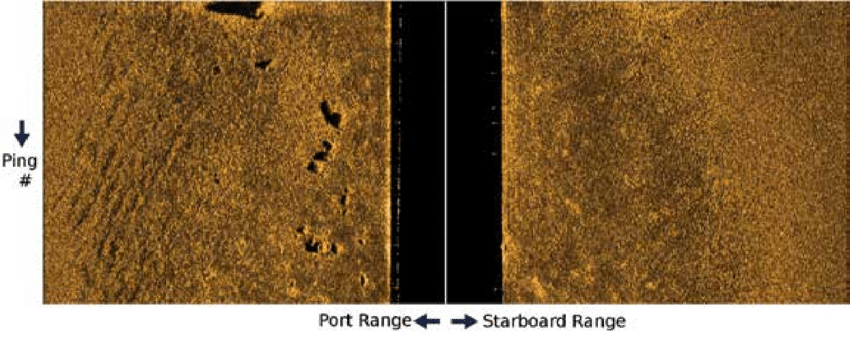
\includegraphics[width=1.0\linewidth]{Pictures/Local_Map_Generation/Swath_Processing/raw_waterfall_image.png}
    \caption{Example of a raw side scan sonar waterfall image showing backscatter intensity versus slant range for consecutive pings. The dark central band corresponds to the sonar blind zone.\textsuperscript{\cite{raw_waterfall_image}}}
    \label{fig:local-map-generation-raw-waterfall-image}
\end{figure}



\subsubsection{Interpolation}
In principle, the vehicle pose and altitude used for swath processing should correspond to the exact ping timestamp. If the navigation solution and altitude measurements are sampled at different times than the sonar ping, interpolation can be used to estimate these quantities at the sonar acquisition instant. This improves temporal alignment between the sonar data and the vehicles estimated motion, which can reduce geometric inconsistencies during later correction stages. In particular, interpolation becomes more relevant for faster vehicle motion, stronger maneuvers, or larger differences between sonar and navigation update rates.

\newpage

\noindent
Let $t_s$ denote the sonar ping timestamp, and let $t_k \leq t_s \leq t_{k+1}$ be two surrounding navigation or altitude measurement times. A linearly interpolated scalar quantity $x(t_s)$ can then be written as
$$
    x(t_s) = (1-\lambda)\,x(t_k) + \lambda\,x(t_{k+1})
$$
where
$$
    \lambda = \frac{t_s - t_k}{t_{k+1} - t_k}
$$
For orientation, the same idea applies, although in practice quaternion interpolation such as SLERP is often preferred to preserve valid rotational geometry.  
\\ \\
For slowly moving and gently maneuvering AUVs, interpolation may be treated as an optional refinement when supporting sensor streams such as the DVL or state estimator are updated much faster than the swath data, since in such cases the practical benefit can be small and the available computation may be better used elsewhere. However, the usefulness of this step depends on the vehicle and sensor infrastructure. For faster maneuvering platforms, less synchronized sensor streams, or systems where the swath data arrive at rates comparable to the supporting navigation data, interpolation becomes a more relevant choice and can improve the temporal alignment of the processed swaths.



\subsubsection{Pitch and Roll Correction}
Variations in vehicle attitude introduce geometric distortions in side scan sonar data. When the vehicle experiences pitch or roll motion, the sonar transducers no longer maintain their nominal orientation relative to the seabed, and the effective beam direction changes from ping to ping. This changes both the true transducer height above the seabed and the location at which the lower edge of the beam can first intersect the bottom. As a result, the boundary between the water column and the first valid seabed return shifts with vehicle attitude and must be updated for each ping.
\\ \\
In the present formulation, pitch and roll correction is treated as a geometric compensation problem based on the estimated vehicle pose, an altitude measurement, and the known mounting offset of each transducer. Rather than estimating the correction directly from the sonar image alone, the method first computes the true height of each transducer above the seabed and then uses the beam geometry to estimate the first physically valid slant range for the port and starboard channels separately. This gives a compact and implementation friendly formulation that matches the real time processing pipeline used in this work.
\\ \\
The geometric intuition is consistent with Figures \ref{fig:local-map-generation-pitch-correction} and \ref{fig:local-map-generation-roll-correction}. Those figures illustrate how pitch rotates the beam in the vertical along track plane and how roll creates an asymmetry between port and starboard. In the implementation, the same effect is handled through rigid body rotations, the transducer mounting offset is rotated by the current vehicle attitude to obtain the corrected transducer height, and the mounted beam direction is rotated in the same way to recover the first valid seabed intersection direction.
\begin{figure}[H]
    \centering
    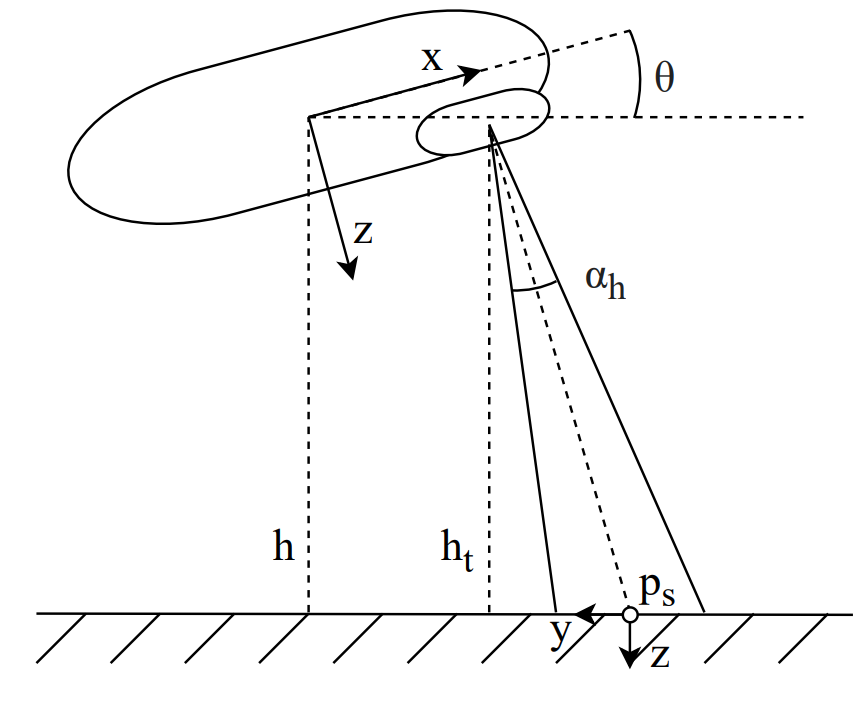
\includegraphics[width=0.75\linewidth]{Pictures/Local_Map_Generation/Swath_Processing/non_zero_pitch.png}
    \caption{Illustration of pitch induced beam rotation. A positive pitch angle $\theta$ changes the effective beam direction and therefore shifts the apparent seabed intersection geometry. The figure is used here as geometric intuition for the rigid body correction model.\textsuperscript{\cite{side_scan_sonar_master_thesis}}}
    \label{fig:local-map-generation-pitch-correction}
\end{figure}
\begin{figure}[H]
    \centering
    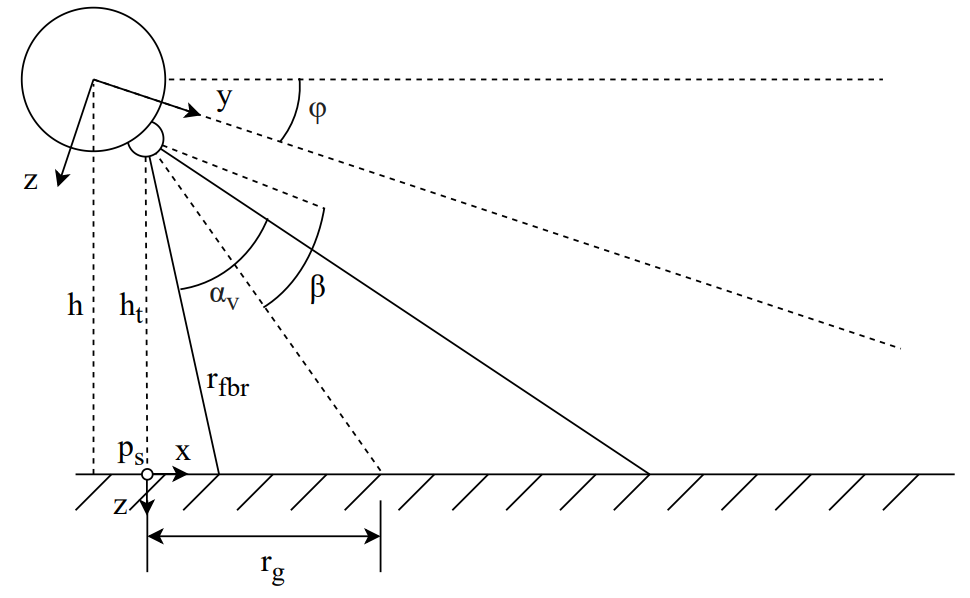
\includegraphics[width=0.75\linewidth]{Pictures/Local_Map_Generation/Swath_Processing/non_zero_roll.png}
    \caption{Illustration of roll induced port starboard asymmetry. A nonzero roll angle $\phi$ changes the effective beam orientation differently for the two channels, which leads to different corrected transducer heights and first valid return ranges.\textsuperscript{\cite{side_scan_sonar_master_thesis}}}
    \label{fig:local-map-generation-roll-correction}
\end{figure}
\noindent
Let the vehicle pose at the sonar ping time be obtained from the state estimate in Equation \ref{eq:kinematics-motion-model-states}, where the quaternion is converted to a rotation matrix using Equation \ref{eq:system-modeling-quaternion-to-so3}. The pose input to the swath processing stage can then be written as $\mathbf{R}_{b}^{n}$. Where $\mathbf{R}_{b}^{n}$ is the rotation from body frame to navigation frame. 
\\ \\
Let the mounting offset of one sonar transducer, expressed in the body frame, be
$$
    \mathbf{p}_{t/b}^b =
    \begin{bmatrix}
        x_t \\ y_t \\ z_t
    \end{bmatrix}
$$
To account for vehicle pitch and roll, this fixed body frame offset is rotated into the navigation frame as
$$
    \mathbf{p}_{t/b}^n = \mathbf{R}_{b}^{n} \mathbf{p}_{t/b}^b
$$
The corrected transducer position relative to the seabed can then be written in full 3D form as
\begin{equation}
    \begin{bmatrix}
        x \\ y \\ h_t
    \end{bmatrix}
    =
    \begin{bmatrix}
        0 \\ 0 \\ h_{\mathrm{DVL}}
    \end{bmatrix}
    -
    \mathbf{p}_{t/b}^n
    \label{eq:local-map-generation-transducer-height-corrected}
\end{equation}
where $h_{\mathrm{DVL}}$ is the altitude measurement referenced to the vehicle body origin. Although Equation \ref{eq:local-map-generation-transducer-height-corrected} is written in full 3D form, only the vertical component $h_t$ is needed in the present swath processing stage, since the goal here is to determine the corrected transducer height above the seabed. This equation is evaluated independently for the port and starboard transducers to obtain $h_{t,\mathrm{port}}$ and $h_{t,\mathrm{stb}}$, which are then used in the following step to compute the first physically valid slant range for each channel.
\\ \\
Once the corrected transducer height $h_t$ has been obtained from Equation \ref{eq:local-map-generation-transducer-height-corrected}, the next step is to estimate the first physically valid slant range along the sonar beam. This corresponds to the first point where the lower edge of the beam can intersect the seabed. The beam center direction of the transducer, expressed in the transducer frame, is defined as
$$
    \mathbf{b}_{c/t}^t =
    \begin{bmatrix}
        0 \\ 1 \\ 0
    \end{bmatrix}
$$
which reflects that the side scan transducer points laterally in its own local frame. Since the first valid seabed return occurs at the lower edge of the vertical beam rather than at the beam center, this direction is rotated by half of the vertical beamwidth $\alpha$:
$$
    \mathbf{b}_{\ell/t}^t = \mathbf{R}_x\!\left(\frac{\alpha}{2}\right) \mathbf{b}_{c/t}^t
$$
where $\mathbf{R}_x\!\left(\frac{\alpha}{2}\right)$ is the rotation from the beam centerline to the lower beam edge. 
\\ \\
To express this lower edge beam direction in the navigation frame, the vehicle attitude and the fixed transducer mounting orientation are combined. Let $\mathbf{R}_{t}^{b}$ denote the fixed rotation from transducer frame to body frame, obtained from the known transducer mounting orientation. The corresponding lower edge beam direction in the navigation frame is then
$$
    \mathbf{b}_{\ell/t}^n = \mathbf{R}_{b}^{n}\mathbf{R}_{t}^{b}\mathbf{b}_{\ell/t}^t
$$
This vector describes the actual lower edge beam direction after both vehicle attitude and transducer mounting have been applied. Its vertical component determines how much downward motion is achieved per unit slant range. Defining the downward fraction as
$$
    d = \left| 
    \begin{bmatrix}
        0 & 0 & 1
    \end{bmatrix}
    \mathbf{b}_{\ell/t}^n
    \right|
    \label{eq:local-map-generation-down-component}
$$
the first physically valid slant range is obtained directly from the right triangle relation between vertical drop and beam length
\begin{equation}
    r_{fbr} = \frac{h_t}{d}
    \label{eq:local-map-generation-first-bottom-return}
\end{equation}
where $h_t$ is the corrected transducer height from Equation \ref{eq:local-map-generation-transducer-height-corrected}. In simple terms, Equation \ref{eq:local-map-generation-first-bottom-return} states that the first valid return range is the slant distance required for the lower edge of the beam to drop vertically by exactly the corrected transducer height. This equation is evaluated independently for the port and starboard channels using their respective mounting orientations and corrected transducer heights, giving $r_{fbr,\mathrm{port}}$ and $r_{fbr,\mathrm{stb}}$. These values are then used in the following blind zone removal step to determine which sonar bins can physically correspond to valid seabed returns.



\subsubsection{Blind Zone Removal}
\begin{figure}[H]
    \centering
    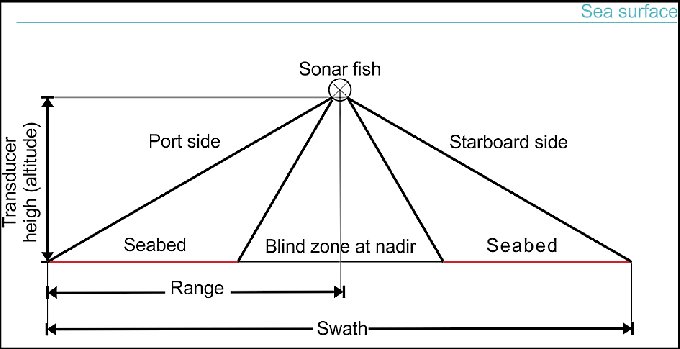
\includegraphics[width=0.80\linewidth]{Pictures/Local_Map_Generation/Swath_Processing/blind_zone_example.png}
    \caption{Transverse view of a side scan sonar geometry showing the blind zone at nadir. The blind zone is the near-vertical region beneath the sonar where no valid seabed echoes are received, separating the port and starboard swaths.\textsuperscript{\cite{blind_zone_example}}}
    \label{fig:local-map-generation-blind-zone-example}
\end{figure}
\noindent
After the geometric correction step, the corrected first valid slant ranges $r_{fbr,\mathrm{port}}$ and $r_{fbr,\mathrm{stb}}$ are available for the two sonar channels. These values define the earliest slant ranges at which the lower edge of the beam can physically intersect the seabed. All samples located closer to the transducer than this limit must therefore belong to the water column or other non seabed returns, and are removed before further processing.
\\ \\
Let the raw swath contain $N_s$ samples per beam and let the maximum recorded slant range be $r_{\max}$. The slant range resolution of one sample bin is then
$$
    \Delta r = \frac{r_{\max}}{N_s}
$$
Using this resolution, the corrected first valid slant range can be converted from meters into a discrete sample index. For one channel, the corresponding first valid bin is written as
\begin{equation}
    k_{fbr} = \left\lfloor \frac{r_{fbr}}{\Delta r} \right\rfloor
    \label{eq:local-map-generation-first-bottom-return-bin}
\end{equation}
where $r_{fbr}$ is obtained from Equation \ref{eq:local-map-generation-first-bottom-return}. In practice, this index is evaluated independently for the port and starboard channels, giving $k_{fbr,\mathrm{port}}$ and $k_{fbr,\mathrm{stb}}$.
\\ \\
The blind zone removal step then masks all bins that lie between the transducer and the first valid bin. Let $I(i)$ denote the raw intensity of one channel at sample index $i$, and let $\tilde{I}(i)$ denote the masked result. In simple terms, all samples before the first valid seabed return are removed, which can be written as
\begin{equation}
    \tilde{I}(i) =
    \begin{cases}
        0, & i < k_{fbr}, \\
        I(i), & i \geq k_{fbr}.
    \end{cases}
    \label{eq:local-map-generation-blind-zone-mask}
\end{equation}
In practice, the implementation applies this masking according to the native storage order of each channel, but the underlying idea remains the same, all bins before the first physically valid seabed return are discarded.
\\ \\
This preserves the original storage order of the channel while removing the near range water column region correctly. In simple terms, the geometric correction step provides the first physically valid return range, Equation \ref{eq:local-map-generation-first-bottom-return-bin} converts that range into a sonar bin index, and Equation \ref{eq:local-map-generation-blind-zone-mask} removes all bins that cannot yet correspond to seabed returns, leaving a cleaner input for the subsequent intensity normalization stage.



\subsubsection{Intensity Normalization}
The received sonar intensity naturally decays with range due to spherical spreading, absorption, beam pattern effects, and other propagation losses. As a result, distant parts of the seabed can appear artificially darker even when their true reflectivity is similar. Intensity normalization is therefore applied to suppress these large scale acoustic effects so that the processed swath better reflects the relative backscatter structure of the seabed.
\\ \\
At this stage, the sonar data have already undergone pitch and roll correction as well as blind zone removal. The remaining signal can therefore be treated as the valid measured backscatter intensity of one swath, where each sample is denoted by $I(i)$. Although these samples now correspond to physically valid seabed returns, they still contain both the true seabed reflectivity and the slowly varying illumination trend introduced by the sonar system and acoustic propagation.
\\ \\
Following the general reflectance illumination formulation used in \cite{side_scan_sonar_master_thesis}, the measured sonar intensity can be modeled as
$$
    I(x, y) = R(x, y) \ast L(x, y)
$$
where $R(x,y)$ represents the underlying seabed reflectivity and $L(x,y)$ represents the slowly varying illumination component. The reflectivity term captures local seabed properties such as roughness, material composition, and grazing angle response, while the illumination term captures larger scale effects such as transmission loss, beam pattern variation, and range dependent attenuation. The aim of intensity normalization is to estimate the illumination component and divide it out so that the remaining signal is dominated more by true seabed structure than by sonar induced brightness variation.
\\ \\
Once an estimate $\hat{L}(x,y)$ of the illumination map is available, the normalized reflectivity estimate can be written as
$$
    \hat{R}(x, y) = \frac{I(x, y)}{\hat{L}(x, y)} = R(x, y) \ast \frac{L(x, y)}{\hat{L}(x, y)}
$$
If $\hat{L}(x,y)$ is a reasonable approximation of the true illumination field $L(x,y)$, then $\hat{R}(x,y)$ becomes a practical estimate of the relative seabed reflectivity. In other words, the normalization removes the dominant low frequency intensity envelope while preserving the local contrast that is more relevant for later mapping and feature extraction.
\\ \\
The illumination map varies slowly across each swath and can therefore be approximated by a low pass estimate of the valid intensity samples. In Haraldstads master thesis, this slowly varying trend was modeled using smoothing cubic splines \cite{side_scan_sonar_master_thesis}. In the present implementation, however, the illumination map is estimated using a lightweight first order IIR low pass filtering approach based on the exponential moving average (EMA), since this is much better suited for real time processing.
\\ \\
A general first order IIR filter can be written as
$$
    y(i) = a\,x(i) + (1-a)\,y(i-1)
$$
where $x(i)$ is the input, $y(i)$ is the filtered output, and $a \in (0,1]$ controls the amount of smoothing. Using the same idea, the illumination envelope of each swath is estimated as
$$
    \hat{L}(i) = \alpha I(i) + (1-\alpha)\hat{L}(i-1)
$$
where $\alpha$ is the EMA smoothing factor. In practice, this filtering is applied independently to each swath and separately for the port and starboard channels. Although this does not produce a perfect illumination estimate, it captures the dominant low frequency trend sufficiently well for the present task while keeping the computational cost low.
\\ \\
After estimating $\hat{L}(i)$, the normalized reflectance profile is computed as
\begin{equation}
    \hat{R}(i) = \frac{I(i)}{\hat{L}(i)}
    \label{eq:local-map-generation-reflectivity-normalization}
\end{equation}
This operation suppresses the large scale illumination effects and produces a more consistent intensity profile across the swath, while retaining the local variations more closely related to actual seabed texture.
\\ \\
The result of this normalization is a swath with a more uniform illumination profile, where artificial range dependent intensity variations are reduced and the seabed structure becomes visually and algorithmically clearer.
\\ \\
Overall, the EMA based normalization provides a practical balance between computational simplicity and correction quality. More advanced illumination estimation methods can in some cases provide a smoother or more globally consistent result, but they are also more computationally expensive. For onboard real time swath processing, the EMA based approach is therefore a suitable and efficient approximation.



\subsubsection{Stacking and Reconstruction}
After each swath has undergone pitch and roll correction, blind zone removal, and intensity normalization, the resulting data provides a cleaner and more consistent representation of the measured seabed backscatter along each ping. To reconstruct a continuous waterfall style image, the processed swaths are stacked sequentially in the temporal order of acquisition. This stacking follows the vehicles forward motion, where each new ping contributes a narrow strip of intensity data along the along track axis.
\\ \\
During stacking, each swath is associated with the estimated vehicle trajectory from the navigation system, which preserves the temporal and spatial consistency of the reconstructed sequence. The along track resolution is mainly determined by the ping rate and vehicle speed, while the across track resolution depends on the sonar sampling in slant range.
\\ \\
The resulting 2D reconstruction forms an improved waterfall image with reduced geometric and radiometric distortion compared to the raw input. This stacked output marks the final stage of swath processing in the present formulation and provides the input for later local map generation and feature extraction.
